\section{Track 3: Dealer Ranking}
Based on the established RFM B2B (Recency, Frequency, Monetary) paradigm, the system categorized the entire network of 798 dealers into 8 strategic segments. These segments were combined with a risk classification model to establish a unified Priority Ranking.

\subsection{Dealer Segment Value Analysis}
To understand the financial implications of these segments, Table \ref{tab:dealer} and Figure \ref{fig:dealer} describe the monetary distribution across the network. Revenue by dealer segment is directly calculated using available monetary metrics from the RFM processing phase.

\begin{table}[H]
\centering
\small
\caption{Dealer Segment Value Summary}
\label{tab:dealer}
\resizebox{\linewidth}{!}{
\begin{tabular}{llllll}
\toprule
\textbf{Segment} & \textbf{Dealer Count} & \textbf{Historical Revenue (VND)} & \textbf{Revenue Share} & \textbf{Avg Revenue per Dealer (VND)} & \textbf{Avg Priority} \\
\midrule
Champions & 91 & 47,412,839,496 & 43.3\% & 521,020,214 & 64.29 \\
At Risk & 190 & 16,904,146,839 & 15.4\% & 88,969,194 & 21.30 \\
Potential & 184 & 16,412,540,750 & 15.0\% & 89,198,591 & 33.04 \\
Loyal & 47 & 14,744,131,882 & 13.5\% & 313,704,934 & 55.62 \\
Big Spender & 21 & 8,617,826,036 & 7.9\% & 410,372,668 & 38.39 \\
Lost & 215 & 4,407,212,836 & 4.0\% & 20,498,664 & 3.12 \\
Hibernating & 32 & 533,687,109 & 0.5\% & 16,677,722 & 7.10 \\
New & 18 & 412,776,491 & 0.4\% & 22,932,027 & 9.06 \\
\bottomrule
\end{tabular}
}
\begin{flushleft}
\footnotesize \textit{Note.} Source: outputs/modeling/phase3\_dealer\_priority\_ranking\_q2\_2026.csv. Segment monetary totals reconcile to the historical revenue total of 109,445,161,439 VND.
\end{flushleft}
\end{table}


\begin{figure}[H]
\centering
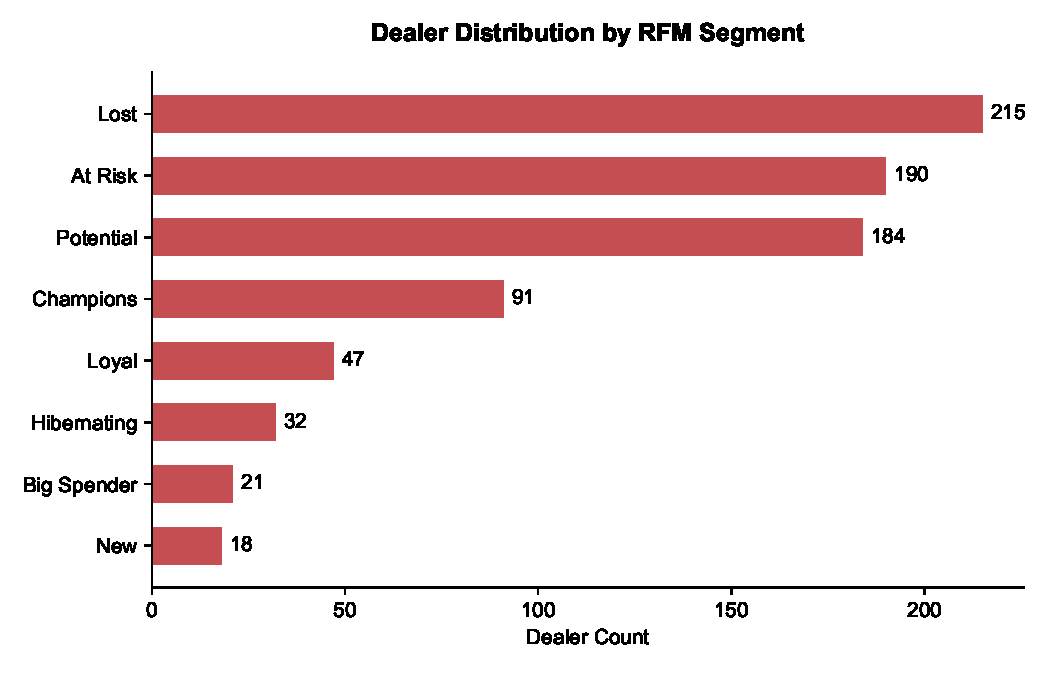
\includegraphics[width=0.85\textwidth]{../figures/en/dealer_segmentation.pdf}
\caption{Dealer Distribution by RFM Segment}
\label{fig:dealer}
\end{figure}

The Champions and Loyal segments act as the primary, stable revenue drivers. The Big Spender demographic requires a dedicated Key Account Care approach, as their purchasing patterns are voluminous but infrequent. Forcing aggressive sales frequency upon this group could prove counterproductive. Conversely, the high volume of Lost and At Risk accounts necessitates immediate reactivation campaigns.

\subsection{Strategic Action Matrix}
To translate these insights into actionable business strategies, Table \ref{tab:dealer_matrix} outlines the recommended approaches and Key Performance Indicators (KPIs) to monitor for each primary segment.

\begin{table}[H]
\centering
\small
\caption{Dealer Action Matrix}
\label{tab:dealer_matrix}
\resizebox{\linewidth}{!}{
\begin{tabular}{lllll}
\toprule
\textbf{Segment} & \textbf{Business Meaning} & \textbf{Risk} & \textbf{Recommended Action} & \textbf{KPI to Monitor} \\
\midrule
Champions & High value, frequent & Low & Retain and protect & Retention rate / Repeat revenue \\
Loyal & Steady buyers & Low & Maintain engagement & Order frequency \\
Big Spender & High value, rare & Medium & Dedicated account care & Total revenue / Account retention \\
Potential & Promising buyers & Medium & Nurture and convert & Conversion to Loyal/Champion \\
At Risk & Dropping frequency & High & Reactivation campaign & Reactivation rate \\
Lost & Inactive long term & Very High & Low-cost reactivation or deprioritize & Response rate \\
Hibernating & Inactive & High & Periodic nurture & Reactivation signal \\
New & Just onboarded & Unknown & Onboarding & Second order rate \\
\bottomrule
\end{tabular}
}
\begin{flushleft}
\footnotesize \textit{Note.} Strategic actions and KPIs tailored to each RFM B2B segment.
\end{flushleft}
\end{table}

\FloatBarrier
